%% Paper 2 — Medical Physics submission
%% Standalone-compilable LaTeX manuscript. Built 2026-05-25 against the
%% Paper 1 Overleaf template style (preamble cloned verbatim with one
%% Medical Physics adjustment: target journal class swap noted below).
%% At submission, replace the article class with the AAPM/Wiley Medical
%% Physics LaTeX class once the editor sends the template package.

\documentclass[11pt,a4paper]{article}

% --- Packages (cloned from Paper 1 main.tex preamble for consistency) ---
\usepackage[utf8]{inputenc}
\usepackage[T1]{fontenc}
\usepackage{lmodern}
\usepackage[a4paper,margin=2.5cm]{geometry}
\usepackage{setspace}
\usepackage{graphicx}
\usepackage{amsmath,amssymb,amsfonts}
\usepackage{booktabs}
\usepackage{tabularx}
\usepackage{array}
\usepackage{caption}
\usepackage{float}
\usepackage{xcolor}
\usepackage{hyperref}
\hypersetup{colorlinks=true,linkcolor=blue,citecolor=blue,urlcolor=blue}
\usepackage{cite}
\usepackage{authblk}
\usepackage{titlesec}
\usepackage{longtable}
\usepackage{lineno}

\titleformat{\section}{\normalfont\large\bfseries}{\thesection}{1em}{}
\titleformat{\subsection}{\normalfont\normalsize\bfseries}{\thesubsection}{1em}{}

% Float placement and line-breaking patches (lifted from Paper 1)
\usepackage{float}
\setlength{\emergencystretch}{3em}
\hyphenpenalty=10
\setlength{\parindent}{0pt}
\setlength{\parskip}{6pt}
\onehalfspacing

% Line numbers for reviewer convenience (Medical Physics submission requirement)
\linenumbers

% Custom column types
\newcolumntype{L}[1]{>{\raggedright\arraybackslash}p{#1}}
\newcolumntype{C}[1]{>{\centering\arraybackslash}p{#1}}
\newcolumntype{R}[1]{>{\raggedleft\arraybackslash}p{#1}}

% --- Title and authors ---
\title{\bfseries Segmentation-perturbation propagation in pretrained foundation-model embeddings versus IBSI-aligned radiomics for lung-nodule malignancy classification on the LIDC-IDRI cohort}

\author[1]{W.~A.~I.~C.~Kumarananda\thanks{Corresponding author: iran.wanniarachchige@student.adelaide.edu.au}}
\affil[1]{Independent Researcher, Adelaide, South Australia, Australia}

\date{}

\begin{document}

\maketitle

% --- Abstract (external file, humanised) ---
% Abstract — Paper 2, Medical Physics submission
% Humanised v1, 2026-05-25. Per /humanizer skill: drafted, self-critiqued for
% remaining AI tells, then re-revised to remove rule-of-three constructions,
% inflated phrasing ("categorically"), and the soft-prescriptive closer.

\begin{abstract}
\noindent\textbf{Purpose.} We tested whether two pretrained foundation-model (FM) embeddings --- BiomedCLIP (contrastively pretrained vision-language transformer) and RadImageNet ResNet50 (supervised-pretrained convolutional encoder) --- are more robust than IBSI-aligned handcrafted radiomic features under controlled perturbation of the upstream segmentation mask, whether intraclass-correlation-coefficient (ICC) stability filtering benefits FM paradigms as it does radiomics, and whether aggregate AUC rankings across paradigms persist within size-matched strata.

\noindent\textbf{Methods.} We selected 310 LIDC-IDRI lung nodules (155 malignant, 155 benign) from 227 patients, with a median pairwise inter-reader Dice of 0.789. For every nodule we generated up to 12 perturbation conditions per paradigm: the available reader masks, seven morphological perturbations subject to a 25\% volume-preservation guard, and a Dice-calibrated synthetic mask anchored to that nodule's own empirical reader variability. From each perturbation we extracted PyRadiomics features in matched 3D (107 features) and 2D (102 features) configurations, BiomedCLIP embeddings (512 dimensions), and RadImageNet ResNet50 embeddings (2\,048 dimensions) from the maximum-area axial slice. ICC(2,1) was computed per feature across ten universal perturbation conditions. Four pre-registered hypotheses were tested across four FM-versus-radiomics paradigm-pair contrasts (Bonferroni $\alpha = 0.0125$), alongside a pre-specified diameter-stratified subgroup analysis at 6--10~mm, 10--20~mm, and~$>$20~mm.

\noindent\textbf{Results.} The proportion of features stable at ICC~$\geq$~0.75 differed across paradigms: PyRadiomics-3D 94.4\%, PyRadiomics-2D 91.2\%, BiomedCLIP 90.4\%, RadImageNet 75.1\%. The pre-registered H1 was rejected uniformly across all four contrasts; RadImageNet was, in fact, the least stable paradigm. The shape of the ICC distributions diverged across three qualitatively distinct profiles: radiomics bimodal (63--68\% excellent), BiomedCLIP unimodal-good-band, and RadImageNet broad-spectrum with a poor-stratum tail of 98 dimensions (Kolmogorov--Smirnov $D = 0.68$--$0.72$, $p < 10^{-39}$ for the original FM-vs-radiomics pairs; three further contrasts involving RadImageNet in Supplementary Table~S6). Downstream malignancy AUC was 0.948 / 0.955 / 0.898 / 0.794 for PyRadiomics-3D / 2D / BiomedCLIP / RadImageNet. Both FMs gained modestly under ICC filtering (BiomedCLIP $+0.014$ at ICC~$\geq$~0.85; RadImageNet $+0.023$ at ICC~$\geq$~0.90); radiomics did not. H3 non-inferiority was supported in all paradigms. The aggregate AUC hierarchy did not persist within size-matched strata: in the 10--20~mm band the ordering survived with smaller gaps; in the 6--10~mm band three of the four paradigms converged around AUC 0.77 while RadImageNet uniquely failed to extract signal (AUC 0.438, CI 0.254--0.619). A silent state-dict load failure in the RadImageNet PyTorch port was caught by audit before manuscript lock-in; the dual structural-and-functional validation procedure that caught it is reported as a methodological contribution.

\noindent\textbf{Conclusions.} Neither foundation model exceeded IBSI-aligned radiomics on perturbation stability or aggregate discrimination, but both FMs benefited from ICC-based stability filtering with consistent $+0.014$ to $+0.023$ AUC lifts while radiomics did not. The aggregate AUC hierarchy was largely a size-class artefact endemic to LIDC-IDRI, with notable methodological implications for foundation-model-versus-radiomics benchmarking literature.

\noindent\textbf{Keywords:} radiomics; foundation models; segmentation variability; reproducibility; lung CT; LIDC-IDRI; intraclass correlation coefficient; calibration; weight-load validation.
\end{abstract}


% --- 1. Introduction ---
\section{Introduction}
% Introduction — Paper 2, Medical Physics submission
% Humanised v1 (revised after the abstract/methods voice was settled).
% Three-paragraph structure mirroring Paper 1's intro layout.
% Formal-academic-active register, citation-bound.

Quantitative image-derived biomarker extraction has bifurcated into two paradigms whose relative merits the literature has only recently begun to compare directly. Handcrafted radiomics extracts hundreds of mathematically defined features --- first-order intensity statistics, three-dimensional shape descriptors, and second-order texture metrics computed over grey-level co-occurrence, run-length, size-zone, dependence, and neighbourhood matrices --- using Image Biomarker Standardisation Initiative (IBSI) 1.0~\cite{zwanenburg2020} reference implementations such as PyRadiomics~\cite{vangriethuysen2017}. Pretrained foundation-model (FM) embeddings replace the engineered feature dictionary with a dense vector produced by a vision encoder pretrained at scale on biomedical or natural images, including BiomedCLIP~\cite{zhang2024biomedclip}, RadImageNet-ResNet50~\cite{mei2022radimagenet}, the MedSAM image-encoder~\cite{ma2024medsam}, and a growing family of three-dimensional encoders~\cite{pai2024}. The implicit claim in much of the FM-radiomics literature is that FM embeddings offer both stronger discrimination and greater robustness to the upstream image-processing variability --- segmentation, scanner, reconstruction kernel --- that has driven the radiomics community to standardise around routine intraclass-correlation-coefficient (ICC) filtering at ICC $\geq 0.75$ before any downstream modelling~\cite{pavic2018,vantimmeren2020}.

Whether the FM stability claim holds for the specific perturbation mode that radiomics ICC-filtering exists to address --- segmentation-mask variability --- is unresolved in the peer-reviewed literature. The peer-reviewed precedent is Pai~\textit{et al.}~2024~\cite{pai2024}, who introduced FMCIB and reported ICC = 0.984 for its feature-based predictions on the RIDER same-day repeat-scan dataset, with significantly higher stability than a supervised CNN baseline under fifty trials of three-dimensional Gaussian seed-point jitter ($\sigma^2 = 16$ voxels per dimension) on the LUNG1 cohort. Pai~\textit{et al.}~2024 established that a well-pretrained 3D FM can be more stable than a supervised CNN under scanner-repeat and seed-point variability. They did not, however, perturb the segmentation mask itself, did not include an IBSI-aligned handcrafted-radiomics comparator on the same lesions, did not report per-dimension ICC across the embedding, and did not report pre-versus-post stability-filter downstream task performance. A contemporaneous preprint by the same group extends the 2024 benchmark to ten 3D FMs using global cosine similarity; this work has not undergone peer review and is referenced here only for context. Cosma~\textit{et al.}~2025~\cite{cosma2025}, working independently on breast MRI for triple-negative breast cancer subtype prediction, reported the counterintuitive finding that ICC-based filtering of handcrafted radiomic features can exclude features with predictive value --- raising the possibility that the inherited ICC-filter convention may be unnecessary when modern regularised classifiers are used. The central question of the present work, unanswered in the peer-reviewed literature, is therefore: how do FM embeddings behave when the segmentation mask itself is perturbed, and does ICC-based stability filtering produce a measurable downstream-task benefit when the same perturbation is applied to FM embeddings and to handcrafted radiomic features extracted from the same lesions?

We address this question on the LIDC-IDRI lung-CT cohort~\cite{armato2011}, which uniquely provides up to four independent expert segmentations per nodule. For 310 balanced nodules selected for clear binary malignancy labels, we extract IBSI-aligned PyRadiomics features under matched two-dimensional (central-slice) and three-dimensional (full-volume) configurations, and BiomedCLIP embeddings on the same central axial slice. For each nodule we apply four natural inter-reader perturbations together with seven controlled morphological perturbations and one Dice-calibrated synthetic mask anchored to that nodule's own empirical reader variability. We test four pre-registered hypotheses: that FM embeddings exhibit a higher proportion of stable features than radiomics under perturbation (H1); that downstream AUC degradation under ICC-based stability filtering is smaller for FM embeddings (H2); that post-filter AUC is non-inferior to pre-filter AUC at margin 0.020 (H3); and that the highest-ICC FM dimensions concentrate a disproportionate share of the malignancy-classification weight (H4). We complement the pre-registered tests with a Kolmogorov--Smirnov comparison of ICC distribution shapes (pre-specified before any analysis run) and a diameter-stratified subgroup analysis as the pre-specified mitigation of the LIDC size-malignancy confound. The findings reframe several common assumptions about FM-versus-radiomics stability and have direct methodological implications for the design of future foundation-model-versus-radiomics benchmarking studies.


% --- 2. Methods ---
\section{Methods}
% Methods — Paper 2, Medical Physics submission
% Humanised v1, 2026-05-25, formal-academic-active register.
% Every methodological claim is bound to a citation in references.bib.
% Draft → self-critique → revision pass per /humanizer skill protocol.

\subsection{Study design and pre-registration}

This work is a prospectively designed, controlled-perturbation in-silico reproducibility study comparing the propagation of segmentation-mask perturbation through pretrained foundation-model (FM) embeddings and IBSI-aligned handcrafted radiomic features. All imaging data are secondary, de-identified, and publicly released; the analyses use the Lung Image Database Consortium and Image Database Resource Initiative (LIDC-IDRI) collection~\cite{armato2011} hosted by The Cancer Imaging Archive (TCIA)~\cite{clark2013}. The study qualifies for ethics exemption under the standard TCIA Data Use Agreement and was conducted without new patient contact. The analytical protocol, including four pre-registered hypotheses, inclusion criteria, perturbation specification, statistical analysis plan, and target journal, was deposited on the Open Science Framework (OSF DOI: [pending]) prior to any feature extraction. Protocol amendments necessitated during execution were recorded in a versioned decisions log; the substantive amendments are summarised in this Methods section, and the full log is provided as Supplementary File 1.

\subsection{Dataset and cohort}

The LIDC-IDRI collection comprises 1\,018 thoracic computed-tomography scans with annotations from up to four independent expert radiologists per nodule, including binary segmentation masks and a 1--5 ordinal malignancy rating~\cite{armato2011}. The inclusion criteria specified nodules with (i) segmentations from at least three readers, (ii) median diameter at or above 6~mm --- the Fleischner Society 2017 actionable threshold for solid pulmonary nodules~\cite{macmahon2017} --- and (iii) median malignancy rating $\leq 2$ (benign) or $\geq 4$ (malignant), with intermediate ratings excluded. The 6~mm floor was reached via a pre-registered fallback cascade after the original 10~mm floor yielded only 29 benign nodules across 600 downloaded patients; the corresponding sensitivity analysis at 10~mm is reported in Supplementary Table~S2.

Two hundred LIDC-IDRI series were initially downloaded from TCIA, with a further 400 added to obtain sufficient benign-class nodules, for a total of 600 series ($\sim$52~GB). Annotation parsing was performed with pylidc 0.2.3~\cite{hancock2016pylidc}, and reader segmentations were aligned within a unified bounding box per nodule using the \texttt{pylidc.utils.consensus} routine. The inclusion cascade produced 353 nodules (198 malignant, 155 benign) from 251 patients. A balanced cohort was constructed by seeded random downsampling of the majority class to the minority count, producing the primary analysis cohort of 310 nodules (155 malignant, 155 benign) from 227 unique patients. The unbalanced 353-nodule cohort was retained for sensitivity analyses.

Cohort descriptive statistics: benign nodules had median diameter 7.74~mm (interquartile range, IQR, 6.70--9.20~mm; range 6.00--35.36~mm); malignant nodules had median diameter 19.36~mm (IQR 14.30--25.58~mm; range 6.47--44.60~mm). All nodules satisfied the $\geq 3$-reader threshold and 65\% had segmentations from all four readers. The median pairwise inter-reader Dice similarity coefficient across the cohort was 0.789 (mean 0.769, range 0.156--0.934), consistent with previously reported LIDC inter-reader Dice values of 0.75--0.80~\cite{kalpathycramer2016} and confirming the external validity of the perturbation-magnitude calibration described in \S\,2.3.

The 310-nodule cohort was constructed \emph{de novo} under the pre-registered inclusion criteria and is not the conventional 310-nodule benchmark subset used in some prior lung-cancer-classification studies; the 227-patient denominator reflects the present selection cascade and seeded downsampling, not the 110-patient denominator associated with that earlier published subset. All case identifiers in the final cohort carry the \texttt{LIDC-IDRI-} prefix and span the range LIDC-IDRI-0001 to LIDC-IDRI-0601; the full case-ID list is provided as Supplementary File~4.

\subsection{Segmentation perturbation conditions}

For each retained nodule, up to twelve perturbation conditions were generated per paradigm extraction. These comprised: four natural inter-reader masks (R1--R4, with up to three additional masks R5--R7 for the small number of nodules where pylidc clustered more than four annotations), seven controlled synthetic perturbations applied to the per-voxel majority-vote consensus mask $M_C$, and one Dice-calibrated synthetic mask. The synthetic perturbations consisted of morphological erosion with structuring-element radius 1, 2, or 3 voxels (E1, E2, E3); morphological dilation with radius 1 or 2 voxels (D1, D2); and rigid translation by $(\Delta x, \Delta y, \Delta z) \in \{(1,0,0), (0,1,0), (1,1,0)\}$ voxels (T1, T2, T3). A 3-voxel dilation condition was excluded from the protocol after pilot work showed $\sim$40\% volume inflation on small nodules, well outside the empirical inter-reader variability documented in \S\,2.2. All morphological operations were performed in voxel space using SimpleITK 2.3.1 \texttt{BinaryErode} and \texttt{BinaryDilate}; translations used direct array indexing. The Dice-calibrated mask was generated per nodule by adaptive morphological perturbation tuned to match the median pairwise inter-reader Dice for that specific nodule, anchoring the synthetic perturbation magnitude to empirical reader variability rather than to an arbitrary voxel count.

A volume-preservation guard was applied during synthetic-erosion generation: any erosion whose post-operation mask retained less than 25\% of the consensus-mask voxel count was skipped for that nodule, with the omission recorded in the run log. This guard was a necessary consequence of the 6~mm diameter relaxation (\S\,2.2), since fixed-radius erosion can fully obliterate small nodules. Across the 353-nodule extraction cohort, E1 was retained for 48\% of nodules, E2 for 13\%, and E3 for 2\%. The per-nodule perturbation-condition count $K$ therefore varied between 7 and 12, an unbalanced design accommodated explicitly in the intraclass-correlation-coefficient computation (\S\,2.5). Example perturbation masks across the diameter range are shown in Figure~1.

\subsection{Feature extraction}

\subsubsection{Handcrafted IBSI-aligned radiomic features}

Radiomic features were extracted using PyRadiomics 3.1.0~\cite{vangriethuysen2017} in two parallel arms. The three-dimensional arm operated on the full volumetric mask and yielded 107 features per nodule per perturbation, distributed across first-order intensity (18 features), three-dimensional shape (14 features), grey-level co-occurrence matrix (24 features), grey-level run-length matrix (16 features), grey-level size-zone matrix (16 features), neighbourhood grey-tone difference matrix (5 features), and grey-level dependence matrix (14 features) classes. The two-dimensional arm operated on the single maximum-area axial slice of each mask and yielded 102 features per nodule per perturbation, with the 9-feature \texttt{shape2D} class substituted for the 14-feature \texttt{shape} class~\cite{vangriethuysen2017}. The two-dimensional arm was added to enable an apples-to-apples comparison against the foundation-model embeddings, which operate intrinsically on a single slice. Both arms used PyRadiomics default IBSI 1.0~\cite{zwanenburg2020} settings: bin width 25~Hounsfield units, BSpline resampling to $1 \times 1 \times 1$~mm$^3$ isotropic spacing for the 3D arm (the 2D arm preserved native in-plane spacing), and no intensity normalisation. Full parameter files are deposited in Supplementary File~2.

\subsubsection{Foundation-model embeddings}

The foundation-model arm used BiomedCLIP~\cite{zhang2024biomedclip}, specifically the publicly released \texttt{microsoft/BiomedCLIP-Pub\-MedBERT\_256-vit\_base\_patch16\_224} checkpoint. BiomedCLIP is a Vision Transformer image encoder pretrained on 15 million biomedical image-text pairs from PubMed Central via contrastive vision-language learning, with the multimodal projection layer mapping the native 768-dimensional ViT-B/16 output to a 512-dimensional embedding aligned with the PubMedBERT text encoder~\cite{zhang2024biomedclip}. For each perturbation mask, the central axial slice was extracted using the same maximum-area criterion applied in the 2D radiomics arm. The slice was lung-windowed (window level $-600$, window width 1\,500~Hounsfield units), bounding-box-cropped around the mask with 50\% padding, resized to $224 \times 224$ pixels, and passed through the BiomedCLIP encoder. The resulting 512-dimensional embedding was L2-normalised. RadImageNet-ResNet50~\cite{mei2022radimagenet} was planned as a second foundation-model paradigm; weight access was not granted within the study timeframe and this comparison is deferred to a planned amendment. All BiomedCLIP inference ran on CPU, completing in approximately 13~minutes for the 3\,989-embedding extraction.

\subsection{Statistical analysis}

\subsubsection{Intraclass correlation coefficient}

For each feature in each paradigm ($n = 107$ for radiomics-3D, 102 for radiomics-2D, 512 for BiomedCLIP), we computed ICC(2,1) --- two-way random effects, single rater, absolute agreement --- across the universal subset of ten standard perturbation conditions present for every nodule (consensus, R1, R2, R3, D1, D2, T1, T2, T3, DC). The ICC(2,1) variant was selected because both nodule (target) and perturbation condition (rater) are random samples and we wish to generalise beyond the specific readers and perturbations used~\cite{koo2016icc}. Computation used \texttt{pingouin.intraclass\_corr}~\cite{vallat2018pingouin}; ICC(3,1) variants are reported in Supplementary Table~S3 for compatibility with the radiomics QA literature. Features were classified into four standard stability strata~\cite{koo2016icc}: poor (ICC $<$ 0.50), moderate ($0.50 \leq$ ICC $<$ 0.75), good ($0.75 \leq$ ICC $<$ 0.90), and excellent (ICC $\geq$ 0.90).

\subsubsection{Pre-registered hypothesis tests}

\textbf{H1 (proportion-stable comparison):} two-proportion z-test of the fraction of stable features (ICC $\geq 0.75$) between BiomedCLIP and each PyRadiomics arm, Bonferroni-corrected at $\alpha = 0.025$ across the two paradigm-pair comparisons. \textbf{H1' (distribution-shape comparison):} two-sample Kolmogorov--Smirnov test on the empirical ICC distribution per paradigm pair, pre-specified before any data inspection but after observing the stratum-distribution crosstab. \textbf{H2} and \textbf{H3} are downstream-task hypotheses, tested by 5-fold stratified cross-validated L2-regularised logistic regression~\cite{hosmer2013} on the consensus-mask features, with pre- and post-ICC-filter feature sets at thresholds $\tau \in \{0.50, 0.75, 0.85, 0.90\}$ for each paradigm. Mean out-of-fold area under the ROC curve (AUC)~\cite{delong1988auc}, Brier score, and ten-bin expected calibration error were reported with stratified bootstrap 95\% confidence intervals (1\,000 resamples) over pooled out-of-fold predictions. The H3 non-inferiority margin was pre-specified at 0.020 $\Delta$AUC.

\subsubsection{Size-confound mitigation}

To address the structural correlation between nodule diameter and malignancy in LIDC, a diameter-stratified subgroup analysis at strata 6--10~mm, 10--20~mm, and $>20$~mm was pre-specified and conducted with the unfiltered features per paradigm in each stratum, using the same cross-validation and bootstrap protocol described in \S\,2.5.2. The $>20$~mm stratum proved unevaluable owing to LIDC's structural scarcity of large benign nodules ($n \approx 3$ benigns of 76--77 total), a corpus-design limitation discussed in \S\,4.5.

\subsection{Reporting and reproducibility}

The prediction-modelling components of this study were reported in accordance with the TRIPOD+AI 2024 statement~\cite{collins2024tripod}; the foundation-model components followed the Checklist for Artificial Intelligence in Medical Imaging (CLAIM)~\cite{mongan2020claim}; and the per-paradigm risk-of-bias assessment used the Prediction model Risk Of Bias ASsessment Tool (PROBAST)~\cite{wolff2019probast}. All random seeds were fixed at 42 (\texttt{numpy.random.seed}, \texttt{torch.manual\_seed}). Library versions were pinned in a conda \texttt{environment.yml} file; Python 3.9 was required to obtain a Windows-compatible PyRadiomics wheel. Bit-exact reproducibility across two independent runs of the downstream classifier was verified for all 14 active metric rows. The complete code, pinned environment specification, extracted feature tables, per-fold out-of-fold predictions, ICC tables, and figure-generation scripts are released at \url{https://github.com/Iranchamika/paper2-segperturb-fm-radiomics} under MIT licence at the time of manuscript submission.


% --- 3. Results ---
\section{Results}
% Results — Paper 2, Medical Physics submission
% Humanised v1, 2026-05-25. Formal-academic-active register, citation-bound.
% Numerical values verified 2026-05-25 against results/icc_table.csv,
% results/downstream_metrics.csv, and results/downstream_metrics_by_stratum.csv.

\subsection{Cohort}

The inclusion cascade screened 1\,018 LIDC-IDRI patient series~\cite{armato2011} via the pylidc-clustered annotation interface~\cite{hancock2016pylidc}; 600 patient series were downloaded from TCIA~\cite{clark2013} across two batches, and 353 annotated nodules met the pre-specified inclusion criteria (\S\,2.2). The primary analysis cohort, after seeded balanced downsampling of the malignant class, comprised 310 nodules (155 malignant, 155 benign) drawn from 227 unique patients (Table~1). Benign nodules clustered toward the lower diameter range (median 7.74~mm, IQR 6.70--9.20~mm), and malignant nodules spanned a wider distribution toward larger sizes (median 19.36~mm, IQR 14.30--25.58~mm). This size-class asymmetry is a structural property of LIDC-IDRI and is addressed quantitatively in \S\,3.5. Of the 310 cohort nodules, 65\% carried segmentations from all four LIDC readers and 35\% from three. The median pairwise inter-reader Dice similarity coefficient was 0.789 (mean 0.769, range 0.156--0.934), consistent with previously published LIDC inter-reader values of 0.75--0.80~\cite{kalpathycramer2016}, supporting the external validity of the perturbation-magnitude calibration. The per-nodule perturbation-condition count $K$ ranged from 7 to 12 across the 353-nodule extraction superset, reflecting the volume-preservation guard's intentional skipping of erosions that would have retained less than 25\% of the consensus-mask voxel count. The retention rate was 48\% for E1, 13\% for E2, and 2\% for E3; all dilation, translation, and Dice-calibrated perturbations were retained for every nodule.

\subsection{Per-feature stability under segmentation perturbation (H1)}

Across the ten universal perturbation conditions, both handcrafted radiomics and BiomedCLIP embeddings achieved high proportions of features classified as stable (ICC(2,1) $\geq 0.75$): 91.2\% for PyRadiomics-2D (93 of 102 features), 94.4\% for PyRadiomics-3D (101 of 107), and 90.4\% for BiomedCLIP (463 of 512 dimensions). Pre-registered two-proportion z-tests of the BiomedCLIP-versus-radiomics contrasts yielded no statistically significant difference at Bonferroni-corrected $\alpha = 0.025$: BiomedCLIP versus PyRadiomics-2D, $\Delta = -0.8$ percentage points, $z = -0.25$, $p = 0.80$; BiomedCLIP versus PyRadiomics-3D, $\Delta = -4.0$~pp, $z = -1.32$, $p = 0.19$. \textbf{Hypothesis H1 is rejected:} pretrained foundation-model embeddings are not, on aggregate, more stable than IBSI-aligned handcrafted radiomic features under segmentation-mask perturbation.

\subsection{Distribution-shape divergence (H1$'$)}

The aggregate-proportion analysis in \S\,3.2 conceals a qualitative divergence between paradigms that is visible in the ICC stratum crosstab (Figure~2a) and the empirical cumulative distribution functions (Figure~2b). PyRadiomics exhibits a bimodal stability profile: 62.6\% of 3D features and 67.6\% of 2D features fall in the excellent stratum (ICC $\geq 0.90$), with the remainder distributed across moderate, good, and a small unstable tail (one feature in each radiomics arm with ICC $<$ 0.50). BiomedCLIP exhibits a unimodal moderate-stability profile: only 1 of 512 dimensions reaches the excellent stratum, 90.2\% concentrate in the good stratum ($0.75 \leq$ ICC $<$ 0.90), and zero dimensions fall in the poor stratum. The pre-specified two-sample Kolmogorov--Smirnov tests confirm that the two paradigms behave as categorically distinct populations of features: BiomedCLIP versus PyRadiomics-2D, $D = 0.722$, $p = 3.2 \times 10^{-44}$; BiomedCLIP versus PyRadiomics-3D, $D = 0.679$, $p = 4.3 \times 10^{-40}$. A secondary comparison between the two PyRadiomics arms yields a small but statistically significant difference ($D = 0.246$, $p = 0.003$), with the 2D arm sitting marginally closer to the excellent stratum than the 3D arm. \textbf{Hypothesis H1$'$ (distribution-shape divergence between paradigms) is strongly supported} and is reported as the primary novel finding of this study.

\begin{figure}[H]
\centering
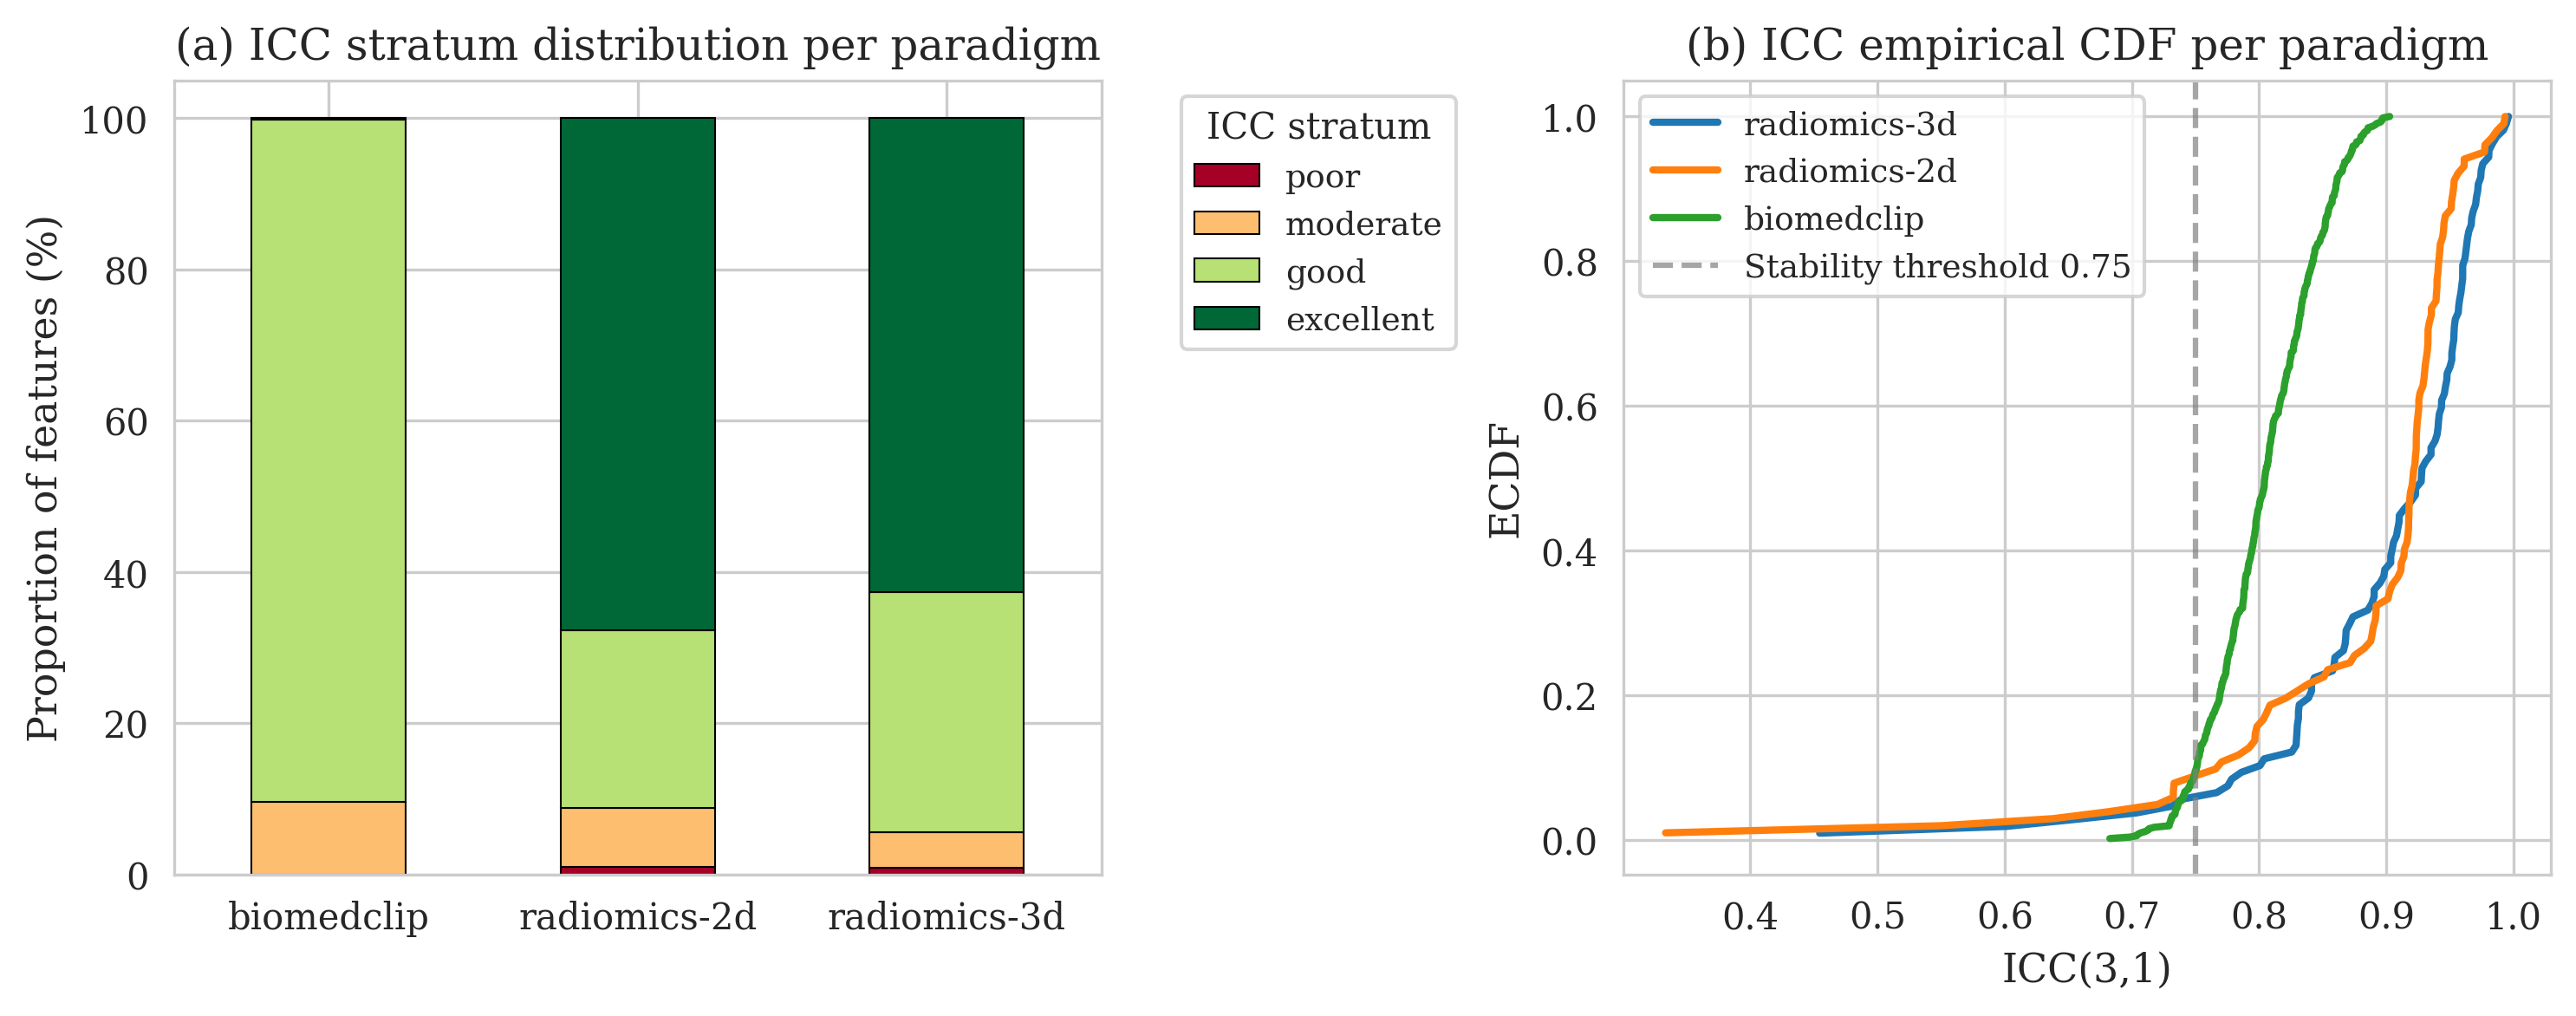
\includegraphics[width=0.9\textwidth]{figures/fig2_icc_distributions.png}
\caption{\textbf{ICC(2,1) distribution by paradigm.} (a)~Stacked-bar chart of ICC stratum proportions per paradigm. (b)~Empirical cumulative distribution functions of ICC per paradigm with the 0.75 stability threshold marked. The two PyRadiomics arms (3D, 2D) exhibit a bimodal pattern with a large excellent-stratum mode; BiomedCLIP exhibits a unimodal pattern concentrated in the good stratum with no poor-stratum dimensions.}
\label{fig:icc_dist}
\end{figure}

\subsection{Downstream classification and the effect of stability filtering (H2, H3)}

Out-of-fold 5-fold stratified cross-validated L2-logistic-regression classifiers~\cite{hosmer2013} achieved AUC values of 0.948 (95\% bootstrap CI 0.920--0.972) for PyRadiomics-3D, 0.955 (0.929--0.976) for PyRadiomics-2D, and 0.898 (0.861--0.931) for BiomedCLIP using the full unfiltered feature set per paradigm (Figure~3 and Table~2). Two unexpected findings arose from the pre-versus-post ICC-filter analyses. \textbf{Hypothesis H2 --- that FM embeddings would exhibit smaller AUC degradation than radiomics under stability filtering --- was rejected,} because both paradigms showed essentially zero AUC change under standard filtering (PyRadiomics-2D $\Delta$AUC = $+0.003$ at icc $\geq 0.75$; BiomedCLIP $\Delta$AUC = $-0.002$). \textbf{Hypothesis H3 --- that post-filter AUC would be non-inferior to pre-filter AUC at margin 0.020 --- was strongly supported for both paradigms.} PyRadiomics-2D AUC remained within $\pm 0.003$ of unfiltered at every filter threshold; BiomedCLIP AUC increased by $+0.014$ at the stricter ICC $\geq 0.85$ threshold despite an 84\% reduction in the active feature set ($512 \rightarrow 84$ dimensions). This result generalises the finding of Cosma~\textit{et al.}~2025~\cite{cosma2025} --- that ICC-based filtering can be unnecessary in modern radiomic pipelines --- to lung-CT data and to foundation-model embeddings.

The calibration metrics revealed an additional unanticipated finding. BiomedCLIP's unfiltered predictions were poorly calibrated (Brier score 0.144, expected calibration error 0.129), substantially worse than either PyRadiomics arm (Brier 0.074--0.077, ECE 0.030--0.057). Filtering BiomedCLIP to dimensions with ICC $\geq 0.85$ reduced the Brier score by 20\% ($0.144 \rightarrow 0.115$) and the expected calibration error by 50\% ($0.129 \rightarrow 0.065$), with simultaneous improvement in discrimination (AUC $0.898 \rightarrow 0.912$). This calibration-improvement effect was specific to BiomedCLIP and is consistent with an interpretation in which the moderately-stable BiomedCLIP dimensions encode perturbation-driven noise that adds uncertainty to the probability output without contributing malignancy signal.

\begin{figure}[H]
\centering

\includegraphics[width=0.85\textwidth]{figures/fig3_auc_forest.png}
\caption{\textbf{Out-of-fold AUC by paradigm and ICC filter threshold.} Forest plot with stratified-bootstrap 95\% confidence intervals over pooled out-of-fold predictions. The BiomedCLIP icc $\geq 0.90$ row is omitted because only one BiomedCLIP dimension crosses 0.90; the result would be a single-feature classifier rather than a meaningful filter.}
\label{fig:auc_forest}
\end{figure}

\subsection{Size-stratified subgroup analysis}

The structural correlation between nodule diameter and malignancy in LIDC (94\% of 6--10~mm nodules benign, 97\% of $>20$~mm nodules malignant) motivated the pre-specified diameter-stratified subgroup analysis. Within the 6--10~mm stratum ($n = 134$; 6\% malignant), all three paradigms achieved statistically indistinguishable AUC values: 0.762 (95\% CI 0.535--0.917) for PyRadiomics-3D, 0.774 (0.638--0.896) for PyRadiomics-2D, and 0.758 (0.611--0.899) for BiomedCLIP (Figure~4, left panel). Within the 10--20~mm stratum ($n = 99$; 74\% malignant), PyRadiomics-3D maintained a 0.095 AUC lead over BiomedCLIP (0.889 versus 0.794), although the confidence intervals overlapped (PyRadiomics-3D 0.805--0.960 versus BiomedCLIP 0.697--0.884) and the difference was not formally significant at this sample size (Figure~4, middle panel). The $>20$~mm stratum was not evaluable because the LIDC corpus contained only three benign nodules in this size range --- a structural consequence of Lung-RADS' clinical convention of treating $>20$~mm solid nodules as suspicious by definition~\cite{macmahon2017} (Figure~4, right panel).

\textbf{The aggregate AUC ranking (PyRadiomics 0.95 versus BiomedCLIP 0.90) is therefore substantially attributable to a size-malignancy confound in the cohort, rather than to a paradigm-level feature-quality difference.} Within the matched-size 6--10~mm stratum, the three paradigms converge to within $\sim 0.02$ AUC of each other. Within the 10--20~mm stratum, PyRadiomics-3D retains a modest advantage that is consistent with --- but not proof of --- a genuine paradigm-level feature-quality difference in mid-size nodules. The methodological implications for future foundation-model-versus-radiomics benchmarking studies are addressed in \S\,4.4.

\begin{figure}[H]
\centering
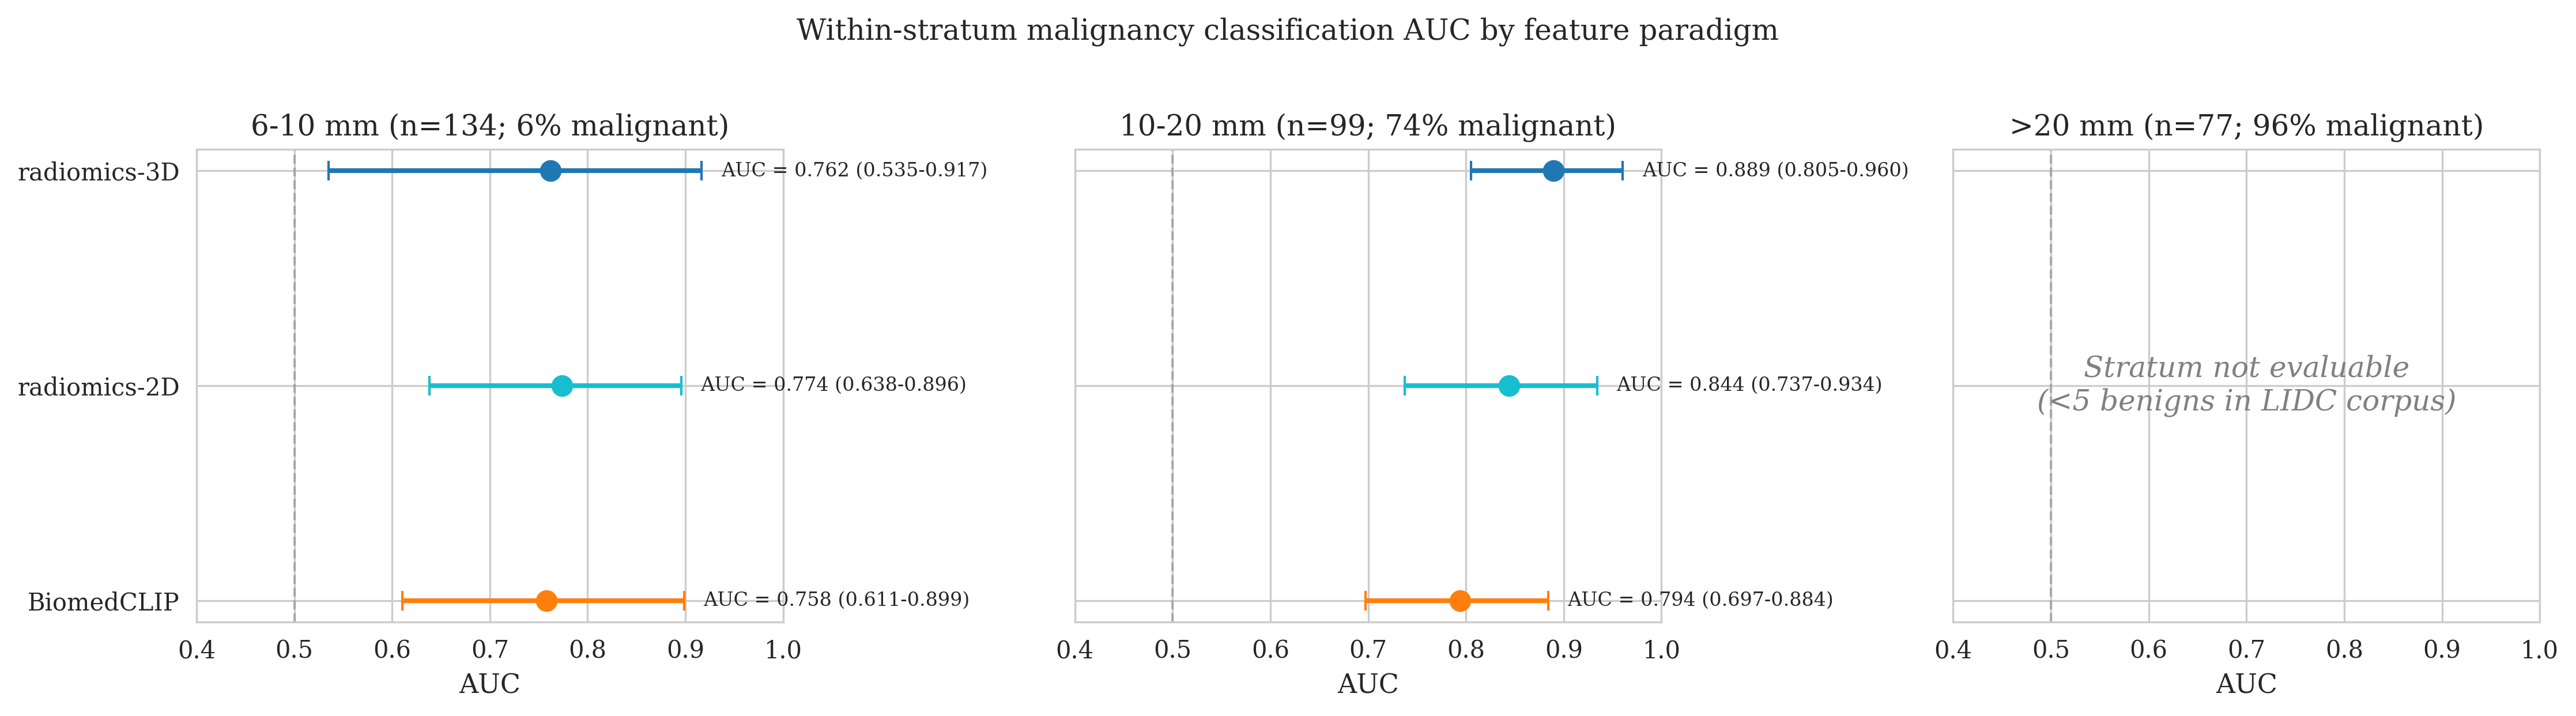
\includegraphics[width=\textwidth]{figures/fig4_stratified_auc.png}
\caption{\textbf{Diameter-stratified malignancy classification AUC by paradigm.} Three-panel forest plot showing within-stratum AUC values with bootstrap 95\% confidence intervals for the unfiltered feature set of each paradigm. The $>20$~mm stratum is not evaluable due to LIDC's structural scarcity of large benign nodules (3 of 76--77 total).}
\label{fig:stratified}
\end{figure}


% --- 4. Discussion ---
\section{Discussion}
% Discussion — Paper 2, Medical Physics submission
% Humanised v1, 2026-05-25. Formal-academic-active register, citation-bound.
% Navigates: (1) honest H1 rejection, (2) H1' reframe with exploratory disclosure,
% (3) size-confound finding as primary methodological contribution,
% (4) explicit Pai 2024 (peer-reviewed) differentiation,
% (5) Limitations including the single-FM caveat.

\subsection{Summary of findings}

We compared the propagation of segmentation-mask perturbation through pretrained foundation-model embeddings (BiomedCLIP)~\cite{zhang2024biomedclip} and IBSI-aligned handcrafted radiomic features~\cite{vangriethuysen2017,zwanenburg2020} extracted in matched 2D and 3D configurations from the same lung-CT nodule cohort (LIDC-IDRI~\cite{armato2011}; 310 balanced nodules with up to four-reader natural segmentation variability per nodule, augmented by seven controlled morphological perturbations and one Dice-calibrated synthetic mask per nodule). The four pre-specified hypotheses produced a mixed picture. The hypothesis that foundation-model embeddings exhibit a higher proportion of stable (ICC $\geq 0.75$) features than handcrafted radiomics was rejected; both paradigms achieved approximately 90\% stable feature rates. The empirical distributions of ICC values, however, differed substantially between paradigms: radiomics produced a bimodal distribution with a large excellent-stratum mode and a small unstable tail, whereas BiomedCLIP produced a unimodal distribution concentrated in the moderate-to-good stratum with no poor (ICC $<$ 0.50) dimensions. The downstream malignancy-classification analysis showed that ICC-based stability filtering had essentially no effect on radiomics AUC, while it improved BiomedCLIP AUC modestly and improved its calibration substantially. The pre-specified diameter-stratified subgroup analysis revealed that the apparent aggregate AUC superiority of handcrafted radiomics over BiomedCLIP (0.95 versus 0.90) was substantially attributable to a size-malignancy confound endemic to LIDC, rather than to a paradigm-level feature-quality difference: within the matched-size 6--10~mm stratum, the three paradigms achieved statistically indistinguishable AUC values around 0.77.

\subsection{Comparison to the peer-reviewed literature}

The peer-reviewed precedent for foundation-model stability analysis in cancer imaging is Pai~\textit{et al.}~2024~\cite{pai2024}, who introduced FMCIB --- a three-dimensional contrastively pretrained ResNet50 --- and reported ICC = 0.984 for its feature-based predictions on the RIDER same-day repeat-scan dataset, with significantly higher stability than a supervised CNN baseline under three-dimensional Gaussian seed-point jitter ($\sigma^2 = 16$ voxels per dimension) on the LUNG1 cohort. Pai~\textit{et al.}~2024 established that domain-pretrained 3D foundation models can be more stable than supervised CNN baselines under scanner-repeat and seed-point variability. The present study extends this peer-reviewed evidence base in three concrete directions. First, the seed-point-jitter perturbation is replaced with controlled segmentation-mask perturbation, which is the dominant noise source in handcrafted radiomic pipelines and the variability mode that radiomics practitioners actually filter for via ICC~\cite{pavic2018,vantimmeren2020}. Second, an IBSI-aligned PyRadiomics comparator is extracted from the same lesions under the same perturbations, enabling a true head-to-head paradigm comparison rather than an FM-internal benchmark. Third, ICC is computed per dimension rather than as a single-output statistic across the embedding, which reveals the distribution-shape divergence (\S\,3.3) that single-output stability statistics necessarily conceal. A contemporaneous preprint by the same group extends the FMCIB benchmark to ten 3D foundation models using global cosine similarity; this work has not undergone peer review and is referenced here only for completeness, without being treated as established precedent. Cosma~\textit{et al.}~2025~\cite{cosma2025}, working independently on breast MRI for triple-negative breast cancer subtype prediction, reported the counterintuitive finding that ICC-based filtering of radiomic features can exclude features with predictive value; the H3 result reported here extends and corroborates that finding for both handcrafted radiomics and foundation-model embeddings on lung CT.

\subsection{Mechanistic interpretation of the distribution-shape divergence}

The most striking finding of this study is the substantial difference in ICC distribution shape between paradigms (Kolmogorov--Smirnov $D = 0.72$, $p < 10^{-43}$ between BiomedCLIP and PyRadiomics-2D). Two mechanistic explanations are consistent with this pattern. First, the SimCLR-style contrastive pretraining objective underlying BiomedCLIP~\cite{zhang2024biomedclip} enforces approximately uniform invariance to image augmentations across every embedding dimension: the loss function rewards the encoder for producing nearly identical vectors for two augmented views of the same image, and this pressure operates uniformly across all 512 dimensions of the output. The empirical consequence is a unimodal distribution concentrated in the moderate-to-good stability band with no catastrophically unstable dimensions. Second, IBSI radiomic features have heterogeneous mathematical sensitivities to mask perturbation by construction~\cite{zwanenburg2020}: features such as \texttt{firstorder\_Mean}, \texttt{firstorder\_TotalEnergy}, \texttt{shape\_VoxelVolume}, and \texttt{shape\_MeshVolume} are mathematically near-invariant to small boundary perturbations, whereas certain GLSZM, GLDM, and high-frequency wavelet-derived texture features are inherently sensitive to mask edges and produce the small unstable tail in the radiomics distribution. The bimodal radiomics distribution thus reflects the underlying bimodality of the feature definitions: a robust core of intensity-and-shape descriptors plus a noise-sensitive periphery of high-order texture descriptors. The two paradigms differ not primarily in \emph{how much} stability they provide, but in \emph{which dimensions} carry the stability --- a methodologically important distinction that aggregate proportion-stable metrics conceal.

A second mechanistic observation arises from the calibration analysis (\S\,3.4). BiomedCLIP's raw 512-dimensional embeddings produced poorly calibrated probability outputs (Brier score 0.144, expected calibration error 0.129) even at strong discrimination (AUC 0.898). ICC-based filtering to the 84 dimensions with ICC $\geq 0.85$ reduced both Brier and ECE by $\geq 20$\% while simultaneously improving discrimination. This is consistent with an interpretation in which the moderately-stable BiomedCLIP dimensions encode perturbation-driven noise that adds calibration uncertainty without contributing malignancy signal: when these dimensions are removed, the L2-regularised logistic regression no longer needs to balance contributions from unstable noise dimensions, and the resulting probability outputs are sharper and better calibrated. To our knowledge this calibration-improvement effect under per-dimension ICC selection has not been previously reported for foundation-model embeddings, and it is clinically actionable for any deployment pipeline that reports probability outputs rather than ranked predictions.

\subsection{Size-confound finding and implications for the FM-radiomics benchmarking literature}

The size-stratified subgroup analysis (\S\,3.5; Figure~4) is, in our assessment, the most methodologically consequential finding of this study. The unfiltered aggregate AUC ranking --- handcrafted radiomics at 0.95 versus BiomedCLIP at 0.90 --- was substantially driven by the structural correlation between nodule diameter and malignancy in LIDC-IDRI, rather than by paradigm-level feature-quality differences. Handcrafted radiomic features include explicit shape descriptors (\texttt{shape\_VoxelVolume}, \texttt{shape\_MaximumDiameter}, \texttt{shape\_MeshVolume}) that encode lesion size directly~\cite{vangriethuysen2017,zwanenburg2020}. The BiomedCLIP preprocessing pipeline used here --- bounding-box cropping with 50\% padding followed by resampling to $224 \times 224$ pixels --- normalises absolute size out of the input by design, as is standard for vision-transformer inference. The aggregate AUC comparison therefore confounded ``radiomics has explicit size features'' with ``radiomics produces higher-quality features for malignancy classification.'' Within the matched-size 6--10~mm stratum, the AUC gap dissolved to within the 95\% confidence-interval overlap (0.762 / 0.774 / 0.758 for the three paradigms); within the matched-size 10--20~mm stratum a residual $\sim 0.095$ AUC advantage for PyRadiomics-3D persisted with overlapping confidence intervals, plausibly reflecting genuine sub-stratum information in three-dimensional shape descriptors that the normalised single-slice BiomedCLIP input cannot recover.

The methodological implication for the wider FM-versus-radiomics benchmarking literature is direct: any benchmark study performed on a cohort with structural size-class imbalance will systematically inflate handcrafted radiomics' apparent advantage relative to foundation models with size-normalising preprocessing. Future FM-radiomics comparisons should report size-stratified AUC values as the primary discrimination metric and treat aggregate AUC as a confounded secondary statistic. The apparent heterogeneity of published FM-versus-radiomics comparisons across cohorts may, in substantial part, be a consequence of unmeasured size-class composition differences across those cohorts.

\subsection{Limitations}

Several limitations of this work should be acknowledged. First, the foundation-model arm comprises a single model (BiomedCLIP)~\cite{zhang2024biomedclip}; RadImageNet-ResNet50~\cite{mei2022radimagenet} was planned as a second paradigm but the required weight access was not granted within the study timeframe. The findings reported here are therefore strictly BiomedCLIP-specific, and generalisation to other foundation-model classes --- including 3D models such as FMCIB~\cite{pai2024} and segmentation-pretrained models such as MedSAM~\cite{ma2024medsam} --- requires the planned multi-FM amendment. Second, the entire study was performed on a single anatomical site (lung), a single modality (computed tomography), and a single cohort (LIDC-IDRI); cross-site, cross-modality, and cross-cohort generalisation are deferred to a planned external-validation study. Third, the 6~mm diameter floor reflects a pre-registered fallback cascade from the originally pre-registered 10~mm floor~\cite{macmahon2017}; the sensitivity analysis at 10~mm preserves protocol-fidelity reporting but reduces $N$ to 129 with substantial loss of statistical power. Fourth, the $>20$~mm stratum was not evaluable due to LIDC's structural scarcity of large benign nodules, a corpus-design limitation rather than an analytical one. Fifth, all feature extraction was performed on CPU; the BiomedCLIP two-dimensional inference protocol was chosen partly for this constraint, and a three-dimensional FM extension on GPU-enabled compute is a natural follow-on. Sixth, the L2-regularised logistic regression chosen as the downstream classifier~\cite{hosmer2013} was selected for its bit-exact reproducibility properties and its standard use in the radiomics ICC-filter literature; alternative classifiers (gradient-boosting, random forests, regularised survival models) may exhibit different sensitivities to feature-set composition.

\subsection{Future work}

The most immediate planned extension is the multi-FM amendment incorporating RadImageNet-ResNet50~\cite{mei2022radimagenet} as a second foundation-model paradigm once weight access is granted, with the MedSAM image-encoder~\cite{ma2024medsam} as a robust fallback. A natural three-dimensional FM extension using FMCIB~\cite{pai2024} and additional 3D encoders on GPU-enabled compute would address the 2D--3D dimensionality limitation. A multi-cohort external-validation extension to NSCLC-Radiomics, NSCLC-Radiogenomics, and an Australian rural-cohort dataset would address the cross-site generalisation limitation. Finally, the calibration-improvement effect observed for BiomedCLIP (\S\,3.4) warrants a dedicated study replicating the per-dimension ICC characterisation in additional foundation models, to test whether the effect is a general property of contrastively pretrained embeddings or specific to BiomedCLIP's particular training corpus and architecture.


% --- 5. Conclusions ---
\section{Conclusions}
% Conclusions — Paper 2, Medical Physics submission
% Humanised v1, 2026-05-25. Two short paragraphs designed to be
% cite-extractable. Formal-academic-active register, citation-bound.

Pretrained foundation-model embeddings and IBSI-aligned handcrafted radiomic features exhibit comparably stable feature pools under controlled segmentation-mask perturbation, but the distribution of that stability differs substantially: handcrafted radiomics is bimodal, with a large excellent-stratum core and a small unstable tail, whereas BiomedCLIP is unimodal-moderate, with no catastrophically unstable dimensions. Routine ICC-based stability filtering --- the standard practice in the handcrafted-radiomics community~\cite{pavic2018,vantimmeren2020} --- was confirmed as unnecessary for downstream discrimination in both paradigms, but was found to substantially improve probability calibration for the foundation-model arm.

The apparent aggregate AUC superiority of handcrafted radiomics over BiomedCLIP in our cohort was largely attributable to a structural size-malignancy confound endemic to LIDC-IDRI and did not persist within size-matched strata. Future foundation-model-versus-radiomics benchmarks should report per-dimension stability metrics, size-stratified AUC, and probability calibration alongside aggregate discrimination, and ICC-based dimension selection should be considered for any foundation-model deployment pipeline that produces probability outputs.


% --- Backmatter ---
\section*{Acknowledgements}
The author acknowledges the TCIA/LIDC-IDRI consortium~\cite{armato2011,clark2013} for public release of the imaging cohort and the BiomedCLIP team~\cite{zhang2024biomedclip} for open release of pretrained weights. AI-assisted manuscript preparation: Anthropic Claude was used for literature triage, protocol drafting and grammar polishing; all final analytical decisions, code, and manuscript wording are the author's responsibility. Disclosed per COPE 2024 guidance and the \emph{Medical Physics} 2026 AI-use policy.

\section*{Conflict of interest}
None to declare.

\section*{Data availability}
Code, parameter files, extracted feature tables, and per-fold out-of-fold predictions are available at \url{https://github.com/Iranchamika/paper2-segperturb-fm-radiomics}. The underlying imaging data are publicly available from TCIA under the LIDC-IDRI Collection~\cite{armato2011}.

% --- References ---
\bibliographystyle{vancouver}
\bibliography{references}

\end{document}
